\documentclass{article}
\usepackage[preprint,nonatbib]{neurips_2026}
\usepackage[utf8]{inputenc}
\usepackage[T1]{fontenc}
\usepackage{hyperref}
\usepackage{url}
\usepackage{booktabs}
\usepackage{amsfonts}
\usepackage{nicefrac}
\usepackage{microtype}
\usepackage{xcolor}
\usepackage{graphicx}
\usepackage{amsmath}

\title{Phishing Website Detection with Machine Learning:\\
Comparing Three Classifiers Across Two Datasets}

\author{%
  Yousiff Rashwan \\
  NetID: yar24 \quad Section: 08 \\
  Rutgers University, Spring 2026 \\
  \texttt{yar24@scarletmail.rutgers.edu}
}

\begin{document}
\maketitle

\begin{abstract}
Phishing pages are a constant problem on the web, and automated detection is one of the more practical ways to fight them.
This project looks at whether a standard set of URL and page-content features can reliably tell phishing sites apart from legitimate ones.
I compared three classical classifiers and a GRU neural network on two public datasets.
On the PhiUSIIL Phishing URL Dataset (235,795 URLs, 50 features), all four models score essentially perfectly, which says more about the data than the models.
On the UCI Phishing Websites dataset the differences emerge: LR gets F1 = 0.917, DT gets 0.944, GRU gets 0.950, and RF gets 0.974.
A word cloud of feature weights and an error analysis of UCI misclassifications both point to the same problem: pages that look structurally legitimate are the hardest cases for every model.

Code: \url{https://github.com/rashwanyousiff/phishing-detection-ml}

Video: \url{[VIDEO_LINK]}
\end{abstract}

\section{Introduction}

Phishing is one of those attacks that keeps working despite everyone knowing about it.
The attacker builds a page that mimics a bank or email provider, waits for someone to type in their credentials, and that is it.
The Anti-Phishing Working Group counted over 5 million attacks in 2023 alone~\cite{apwg2023}.

If a model can flag a URL before the user clicks through, the attack is stopped before any damage is done.
The tricky part is making sure the model works beyond the benchmark it was trained on.
My goal was straightforward: build a clean ML pipeline, compare several classifiers, and actually test whether the results hold up on a second dataset.
I also wanted to understand what the models are doing, not just report scores.

One thing I did not expect was that all four models would hit essentially perfect scores on the main dataset.
That result is worth thinking about carefully.
The cross-dataset evaluation, error analysis, and word cloud are where the more interesting findings come from.

\section{Related Work}
\label{sec:related}

Early ML approaches to phishing detection focused on URL lexical features: length, IP-address presence, special character counts, and subdomain depth.
Whittaker et al.~\cite{whittaker2010} showed that combining these signals with blacklist lookups already produced solid detection rates.
Later work added content features from the rendered page itself, and Tang and Mahmoud~\cite{tang2021} found that URL plus content features consistently beat URL-only approaches, with tree ensembles performing best.

Zieni et al.~\cite{zieni2023} reviewed over 100 phishing detection papers and noted that models trained on one curated benchmark often fail to transfer to data from a different time period or collection process, which directly motivated my second-dataset evaluation.
The PhiUSIIL dataset~\cite{prasad2024} was built to address gaps in older benchmarks, and Prasad and Chandra showed near-perfect performance with gradient-boosted trees on it---a result I replicate here with all four models.

\section{Data}
\label{sec:data}

\subsection{PhiUSIIL Phishing URL Dataset}

The primary dataset is PhiUSIIL~\cite{uci_phiusiil}, which has 235,795 labeled URLs with 56 columns.
I dropped five text-heavy columns (FILENAME, URL, Domain, TLD, Title) leaving 50 numeric inputs.
The class split is 134,850 phishing (57.2\%) and 100,945 legitimate (42.8\%), close enough to balanced that no oversampling was needed.
There are no missing values and no duplicate rows.

\begin{figure}[ht]
  \centering
  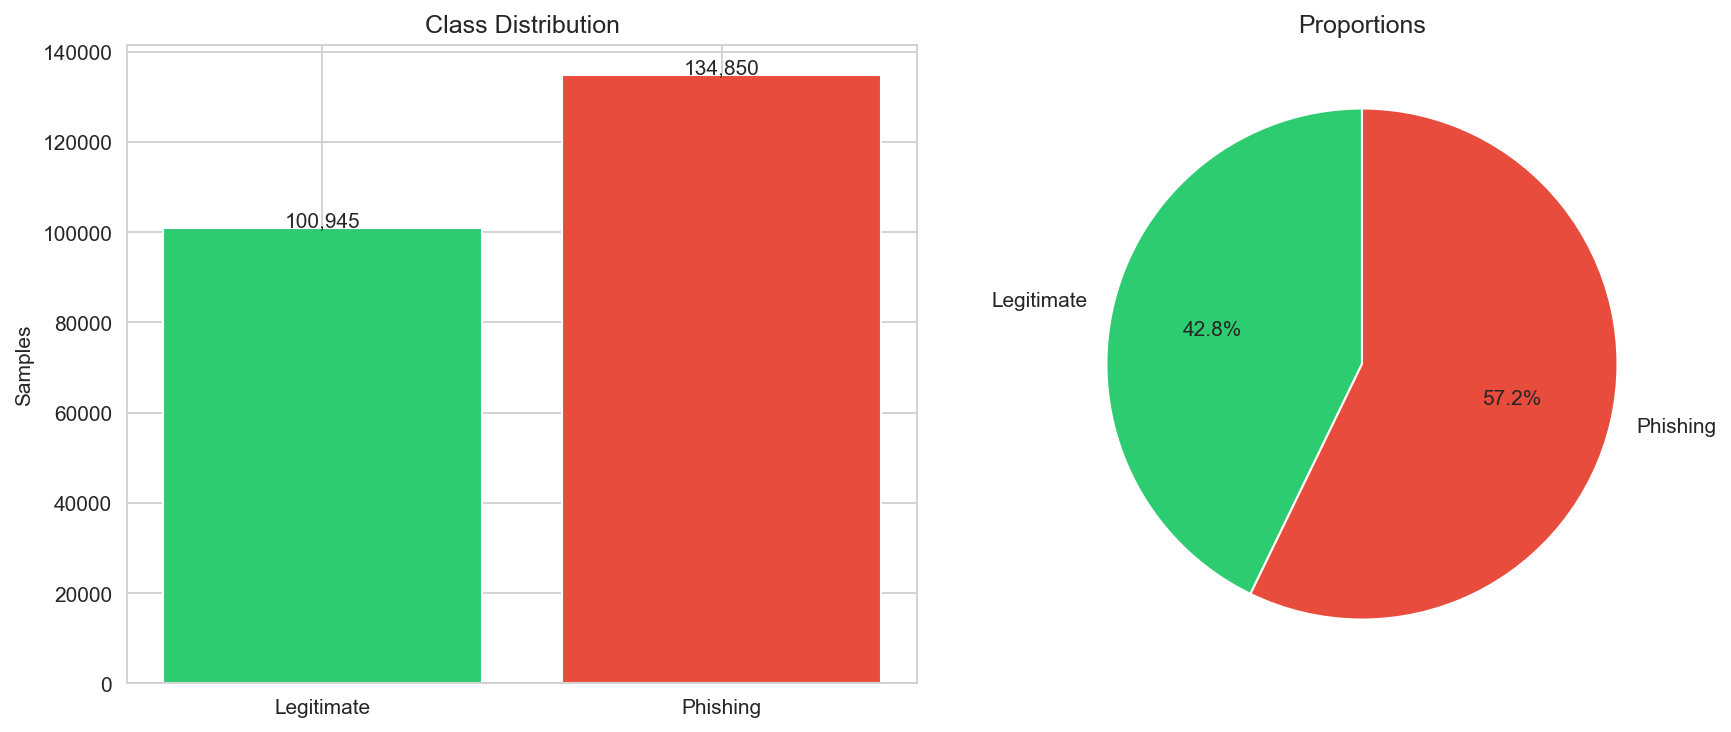
\includegraphics[width=0.66\linewidth]{fig_class_distribution.png}
  \caption{Class distribution in PhiUSIIL. The 57/43 split is close enough to balanced that no resampling was applied.}
  \label{fig:class_dist}
\end{figure}

The 50 features span URL structure (length, domain properties, character ratios, HTTPS flag), page content (image, CSS, JS, iframe counts, form flags, social links, copyright), and broader context (line-of-code count, title-match scores, similarity index, redirect counts, keyword flags).

\subsubsection{Exploratory data analysis}

Figure~\ref{fig:feat_dist} shows distributions of five URL and domain features by class.
\texttt{DomainTitleMatchScore} has the cleanest separation, which makes sense since phishing pages impersonating a brand rarely have a title that actually matches their domain.
Most feature pairs are weakly correlated (Figure~\ref{fig:heatmap}), with \texttt{URLTitleMatchScore} and \texttt{DomainTitleMatchScore} being the clear exception at r = 0.961 since they measure nearly the same thing.

\begin{figure}[ht]
  \centering
  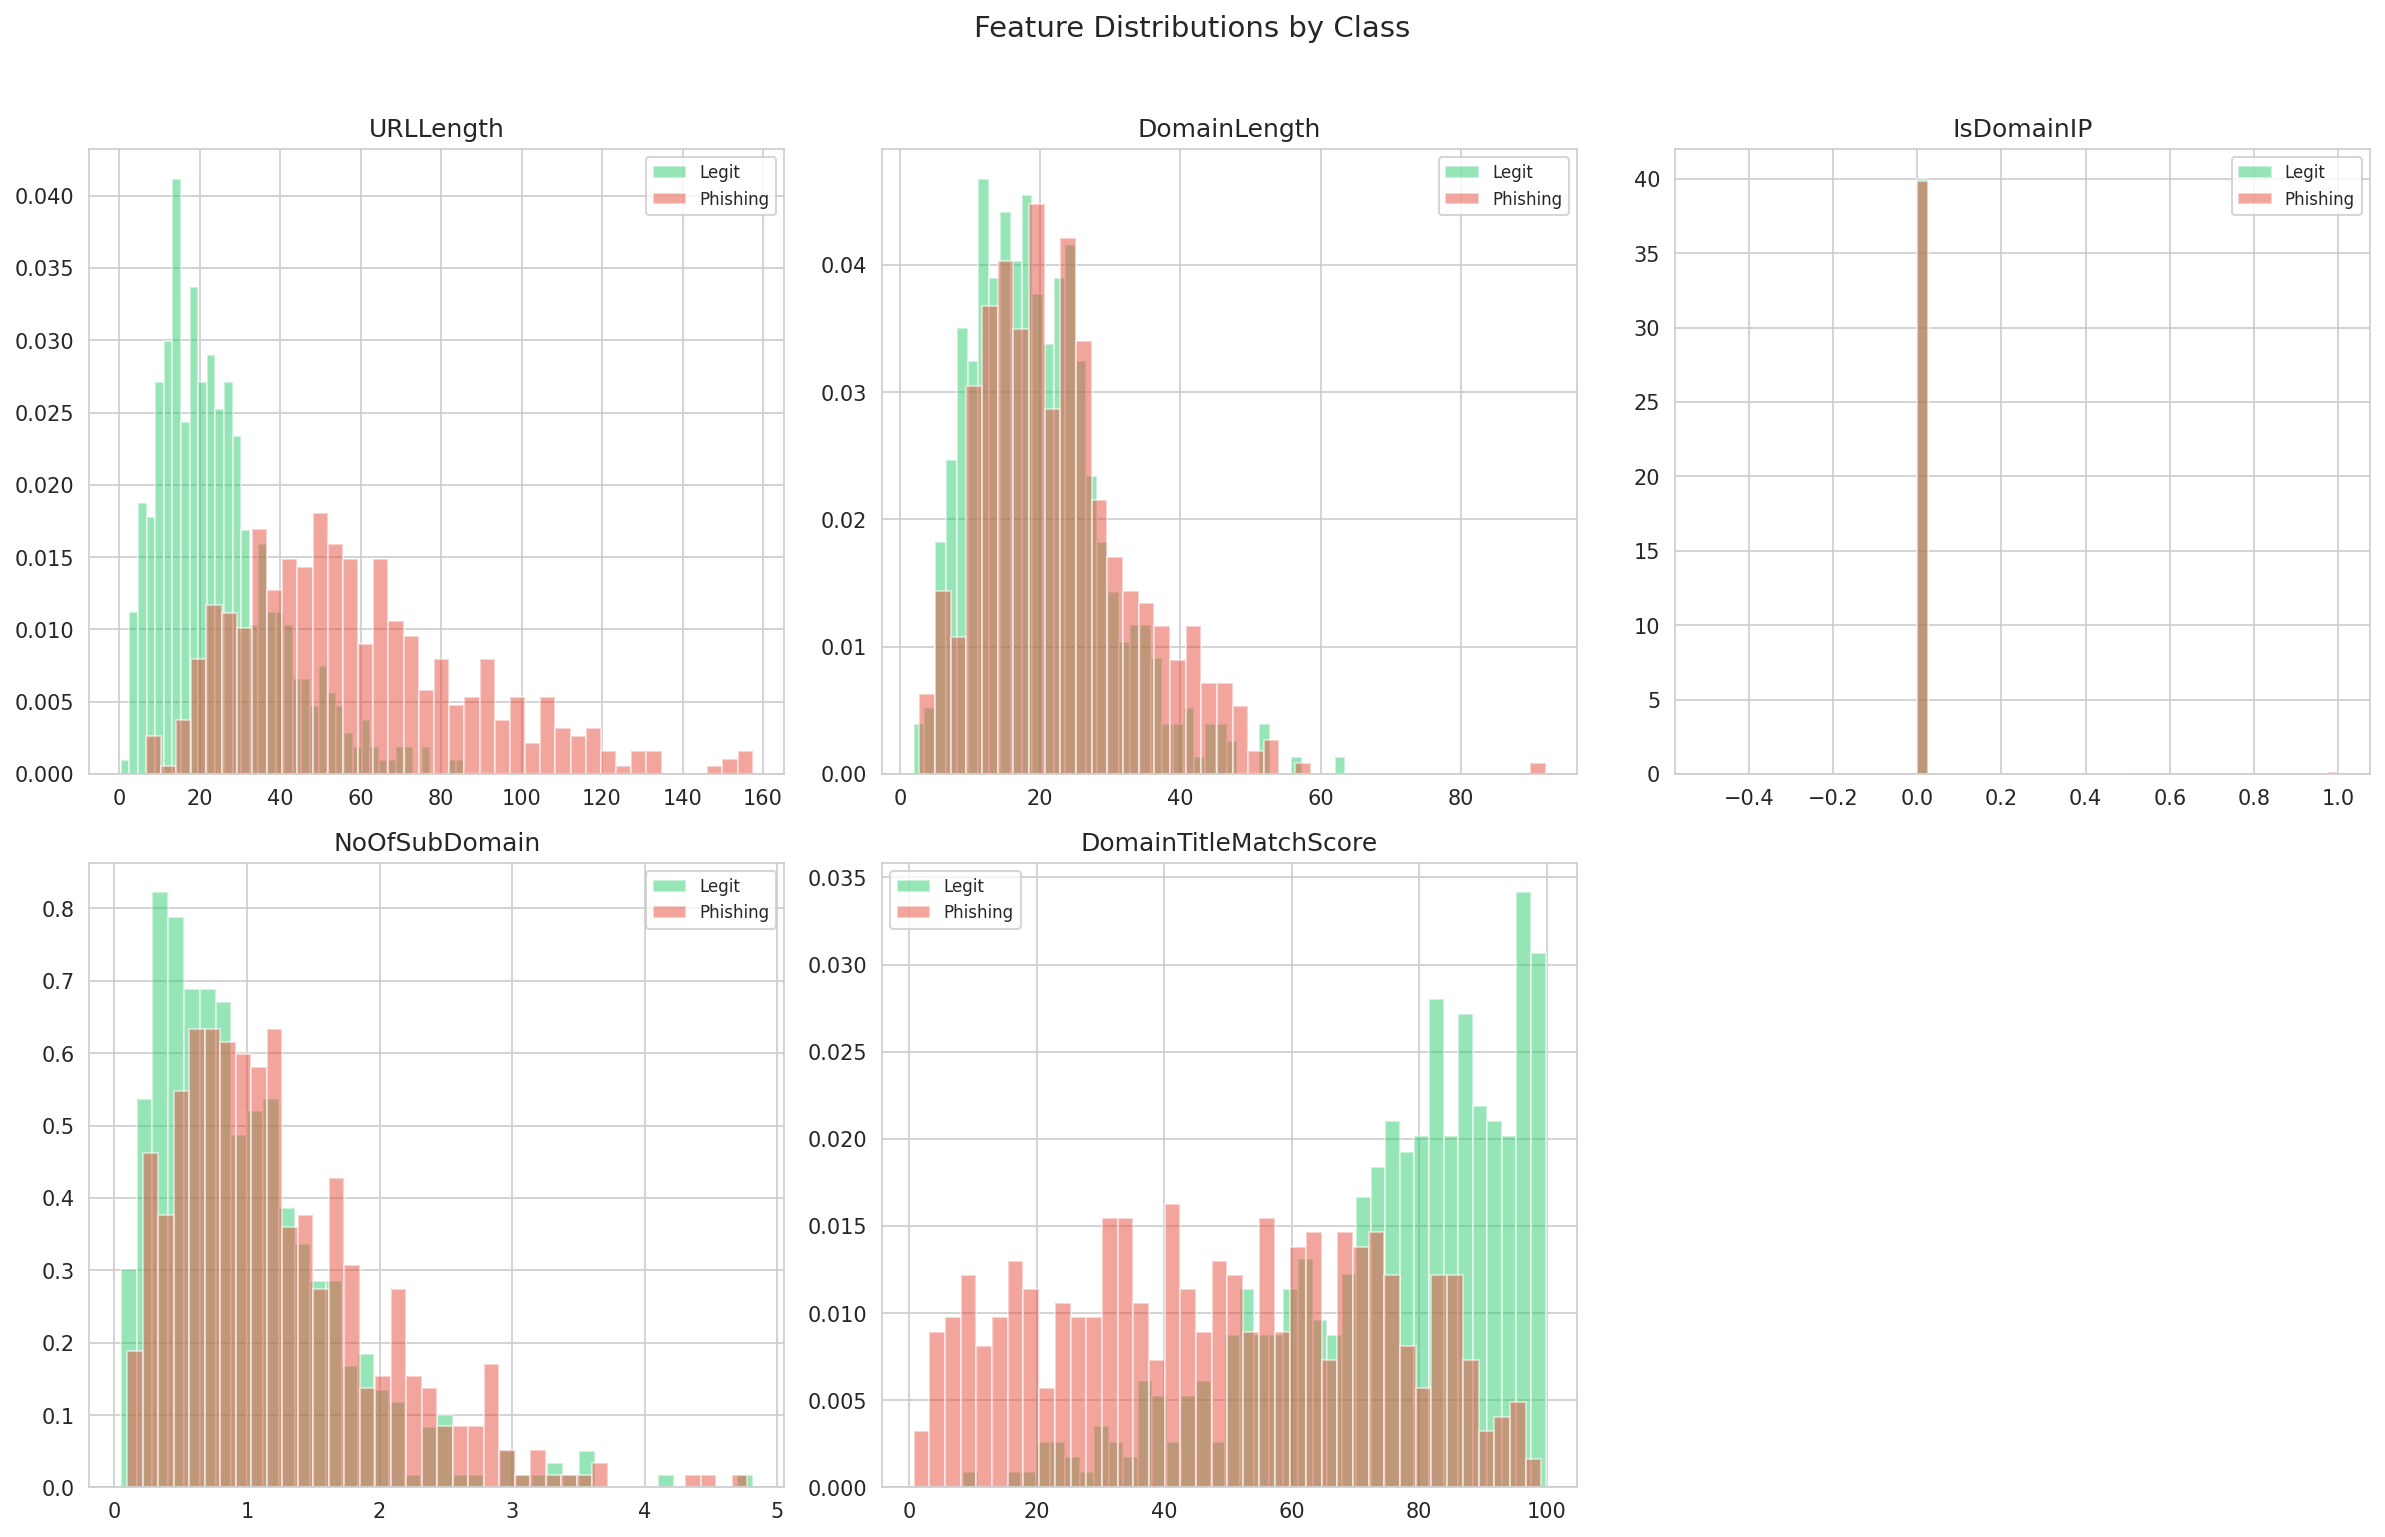
\includegraphics[width=0.86\linewidth]{fig_feature_distributions.png}
  \caption{Distributions of five URL and domain features by class. \texttt{DomainTitleMatchScore} shows the clearest separation.}
  \label{fig:feat_dist}
\end{figure}

Figure~\ref{fig:wordcloud} shows a word cloud of the feature names from the PhiUSIIL Logistic Regression model, sized by coefficient magnitude and colored by direction.
Red and orange features push toward a phishing prediction; green features push toward legitimate.
\texttt{URLSimilarityIndex} dominates the phishing side with a coefficient of $+7.1$, while character-ratio features like \texttt{SpacialCharRatioInURL} and \texttt{LetterRatioInURL} are the strongest legitimacy signals---real URLs tend to be mostly alphabetic with conventional punctuation, whereas phishing URLs often contain random strings or encoded paths.
\texttt{IsHTTPS} appearing as a phishing signal is counterintuitive but reflects that phishing kits routinely obtain free certificates through services like Let's Encrypt.

\begin{figure}[ht]
  \centering
  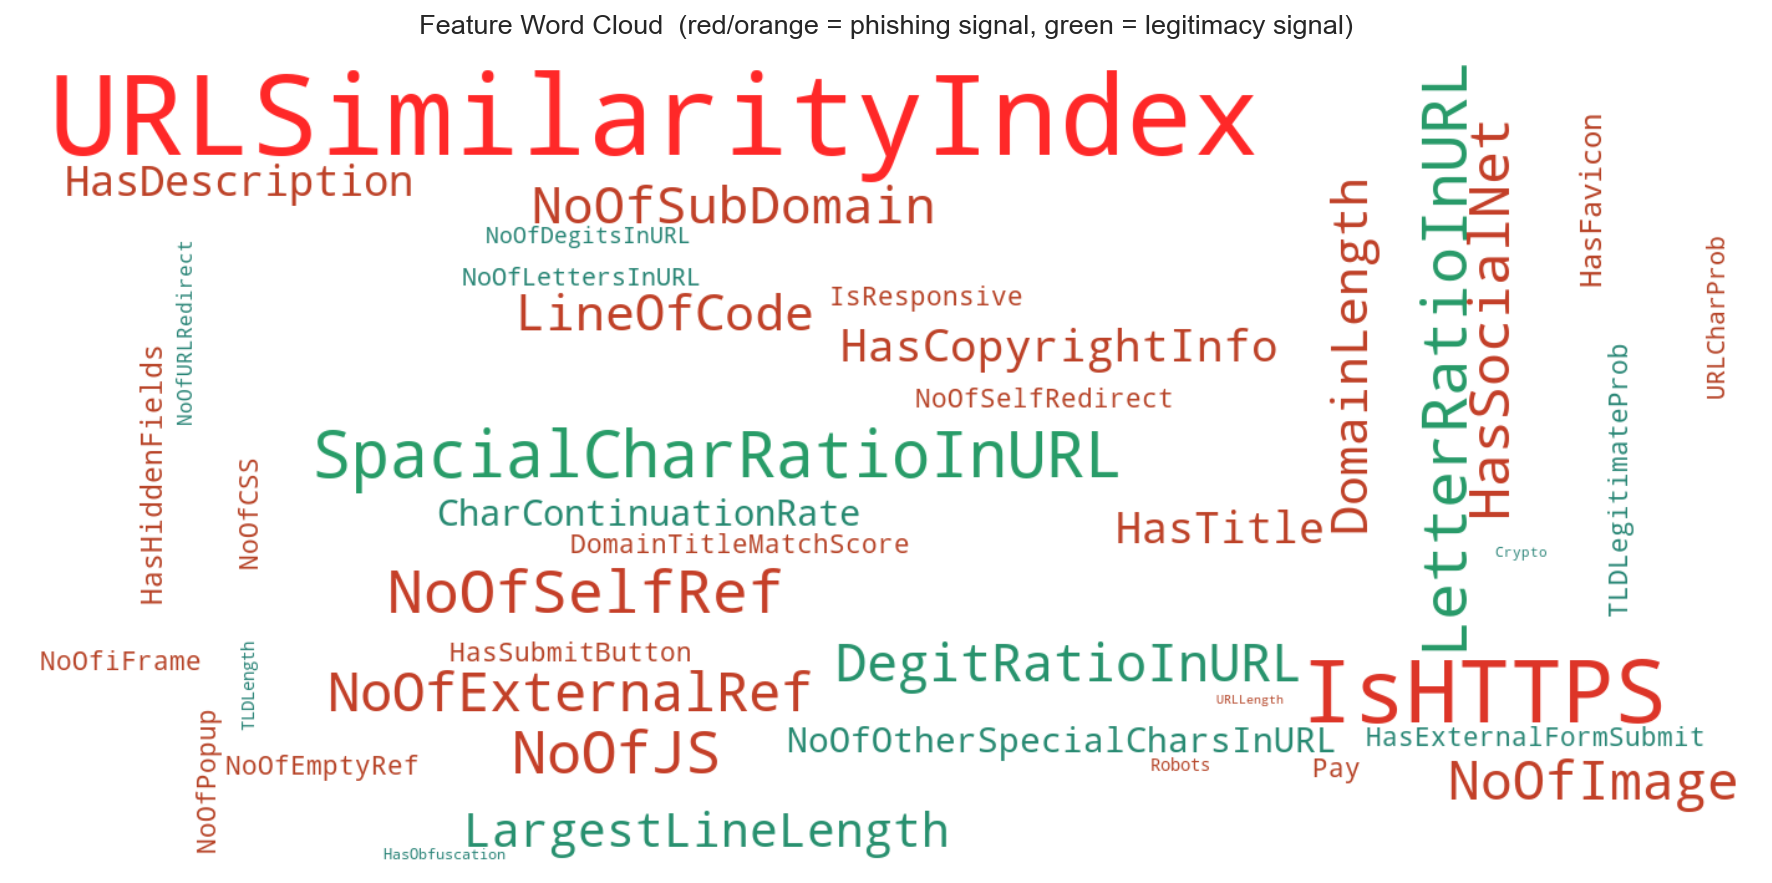
\includegraphics[width=0.56\linewidth]{fig_wordcloud.png}
  \caption{Feature word cloud sized by LR coefficient magnitude. Red/orange = phishing signal; green = legitimacy signal.}
  \label{fig:wordcloud}
\end{figure}

\begin{figure}[ht]
  \centering
  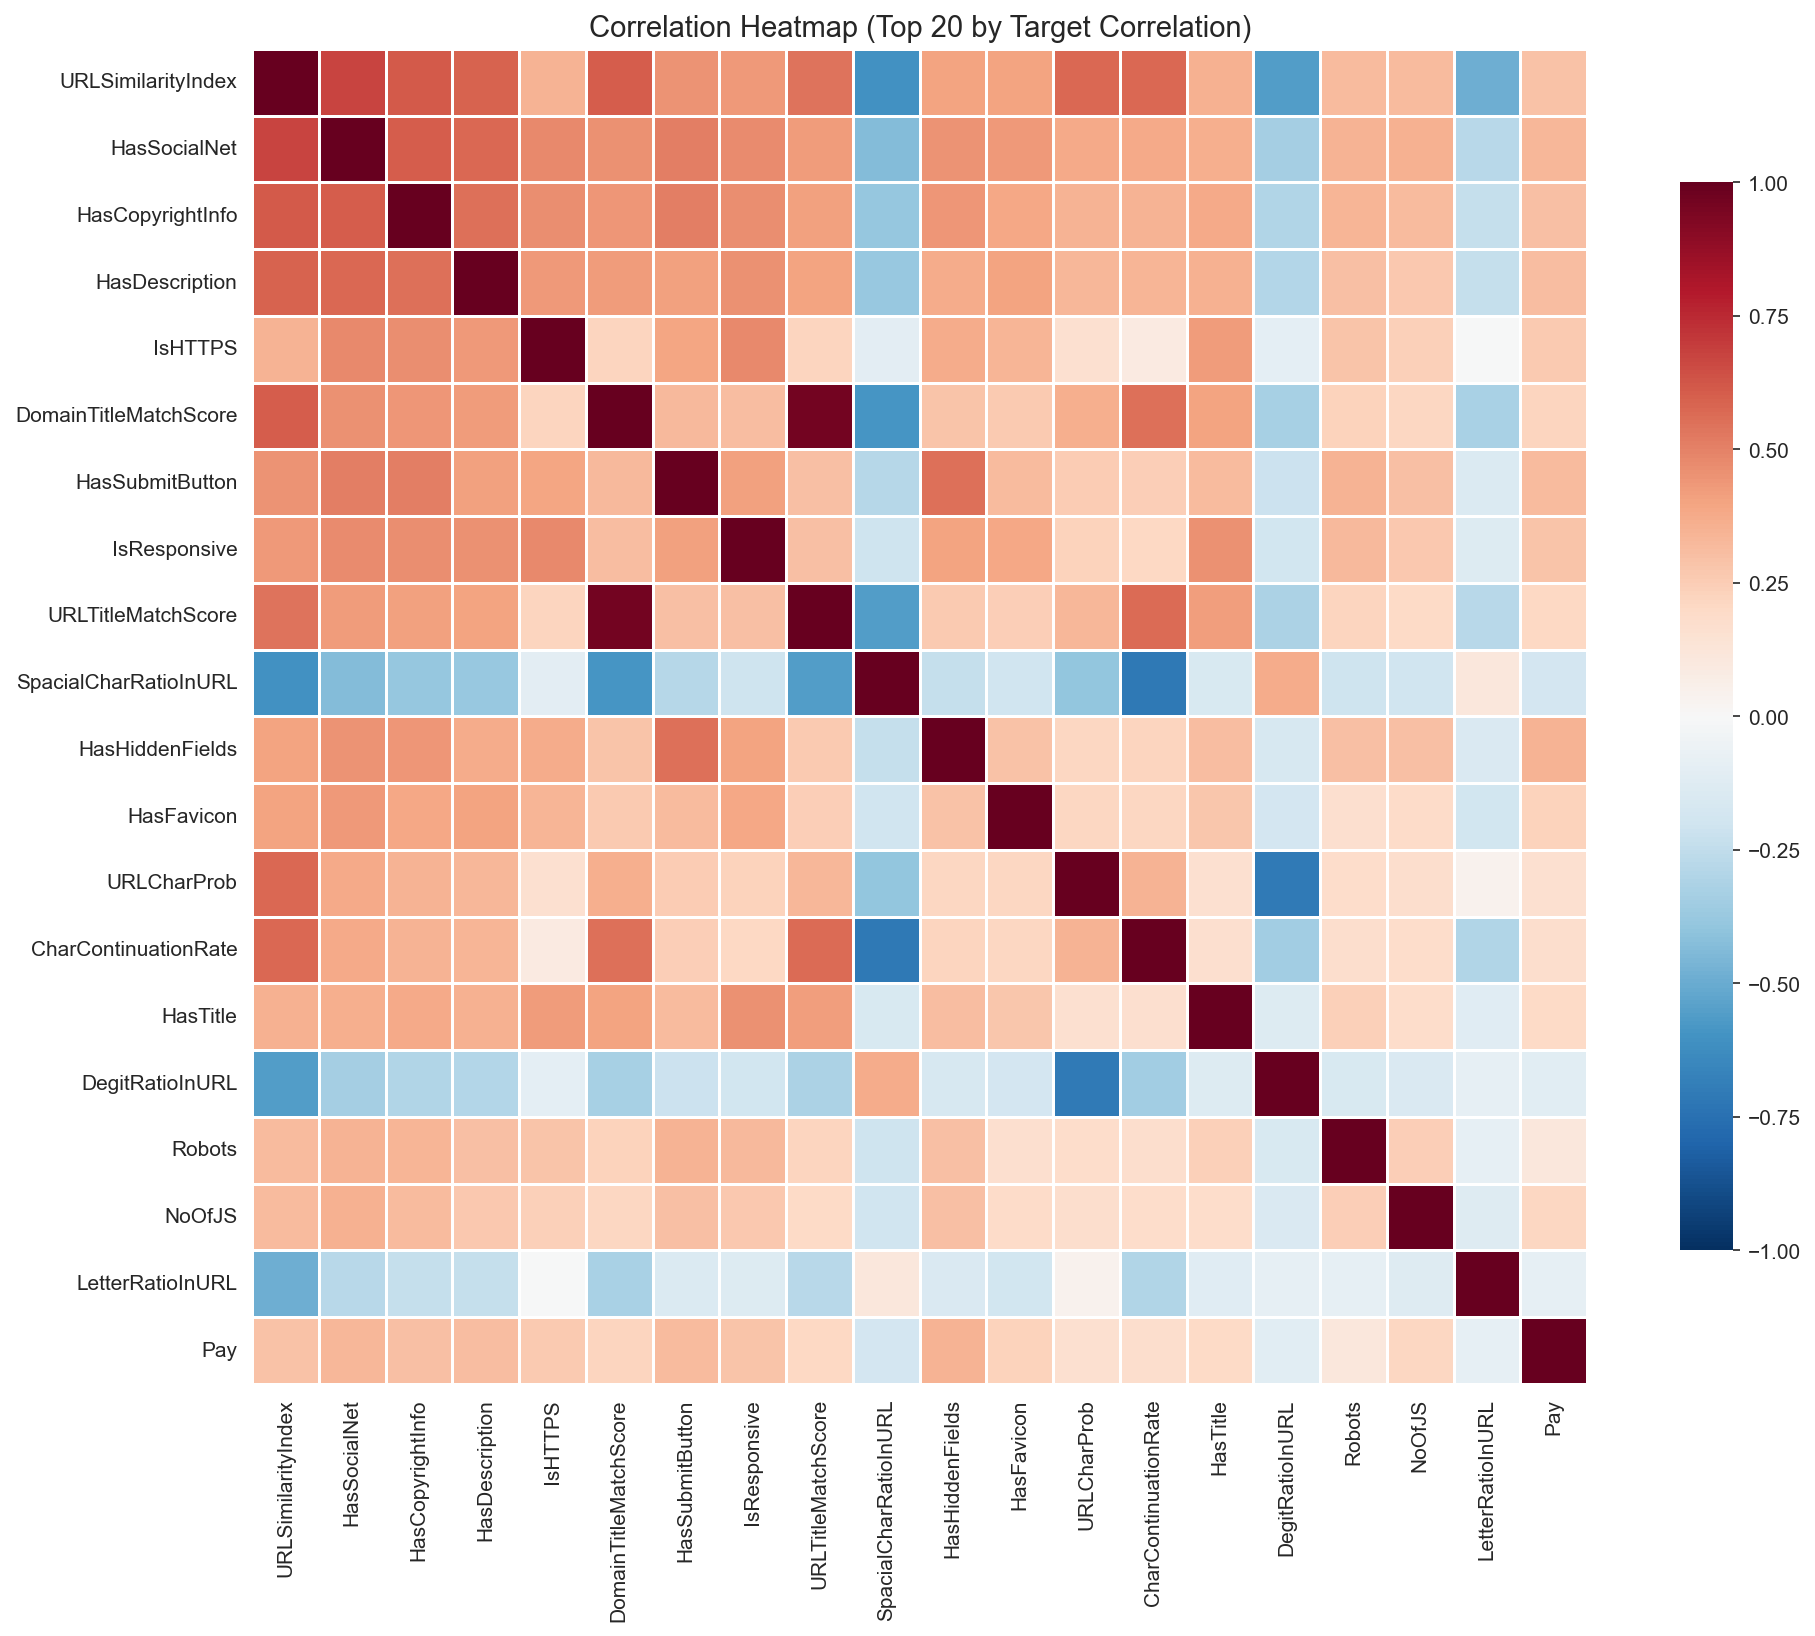
\includegraphics[width=0.82\linewidth]{fig_correlation_heatmap.png}
  \caption{Correlation heatmap for the top 20 features by target correlation. Most pairs are weakly correlated. \texttt{URLTitleMatchScore} and \texttt{DomainTitleMatchScore} stand out at r = 0.961.}
  \label{fig:heatmap}
\end{figure}

\subsection{UCI Phishing Websites Dataset}

For the cross-dataset check I used the UCI Phishing Websites dataset~\cite{uci2015}, loaded from its ARFF file.
It has 11,055 websites with 30 integer features encoded as $\{-1, 0, 1\}$.
After remapping labels to phishing = 1 and legitimate = 0, there are 4,898 phishing and 6,157 legitimate examples.
Models were trained and tested independently on this dataset using the same 80/20 stratified split.

\section{Method}
\label{sec:method}

\subsection{Preprocessing}

All preprocessing runs inside scikit-learn \texttt{Pipeline} objects to prevent leakage.
Logistic Regression uses a \texttt{StandardScaler} step since it is sensitive to feature scale; the tree models do not.
PhiUSIIL split is 80/20 stratified (seed = 42): 188,636 train, 47,159 test.
Class weighting is off since the minority/majority ratio of 0.749 is above the 0.6 threshold I used.

\subsection{Models}

\textbf{Logistic Regression (LR)} models the log-odds of the target as a weighted sum of features, with L2 regularization ($C = 1.0$) and \texttt{max\_iter = 1000}.

\textbf{Decision Tree (DT)} finds the best feature split at each node, capped at \texttt{max\_depth = 10} on both datasets to prevent memorization.

\textbf{Random Forest (RF)} builds 200 trees on bootstrap samples with random feature subsets at each split.
A \texttt{RandomizedSearchCV} tuning pass found $n\_\text{estimators} = 300$, $\text{max\_depth} = 30$, $\text{max\_features} = \sqrt{p}$ optimal, though it matched the default score on PhiUSIIL.

\textbf{GRU} is a small recurrent network~\cite{cho2014} applied to the feature vectors by treating each feature as one timestep.
Two GRU layers (hidden size 64) feed a fully connected head with dropout of 0.3.
I train with Adam ($\text{lr} = 10^{-3}$) and binary cross-entropy for 25 epochs on PhiUSIIL and 50 on UCI.

\subsection{Evaluation}

I report accuracy, precision, recall, F1, and ROC-AUC on the held-out test split for both datasets, alongside 5-fold stratified cross-validation on the training set.

\section{Evaluation}
\label{sec:eval}

\subsection{PhiUSIIL Results}

Table~\ref{tab:phiusiil} shows CV and test results on PhiUSIIL.
All four models are at the ceiling.

\begin{table}[ht]
\caption{PhiUSIIL results ($n_\text{train} = 188{,}636$; $n_\text{test} = 47{,}159$). All models reach the ceiling on this benchmark.}
\label{tab:phiusiil}
\centering
\begin{tabular}{lccccc}
\toprule
Model & CV F1 & Test Acc & Test Prec & Test Recall & Test AUC \\
\midrule
Logistic Regression & 0.9999 & 0.9999 & 0.9998 & 1.0000 & 1.0000 \\
Decision Tree       & 1.0000 & 1.0000 & 1.0000 & 1.0000 & 1.0000 \\
Random Forest       & 1.0000 & 1.0000 & 1.0000 & 1.0000 & 1.0000 \\
GRU                 & 0.9999 & 0.9999 & 0.9999 & 0.9999 & 1.0000 \\
\bottomrule
\end{tabular}
\end{table}

The ROC curves in Figure~\ref{fig:roc} all sit flush against the upper-left corner.
DT and RF are error-free on the test set; LR makes 6 false positives and zero false negatives; GRU makes a handful of errors in both directions.
When even a linear model scores perfectly, the dataset has a dominant separating signal, not just a strong model.
\texttt{URLSimilarityIndex} is almost certainly that signal.

\begin{figure}[ht]
  \centering
  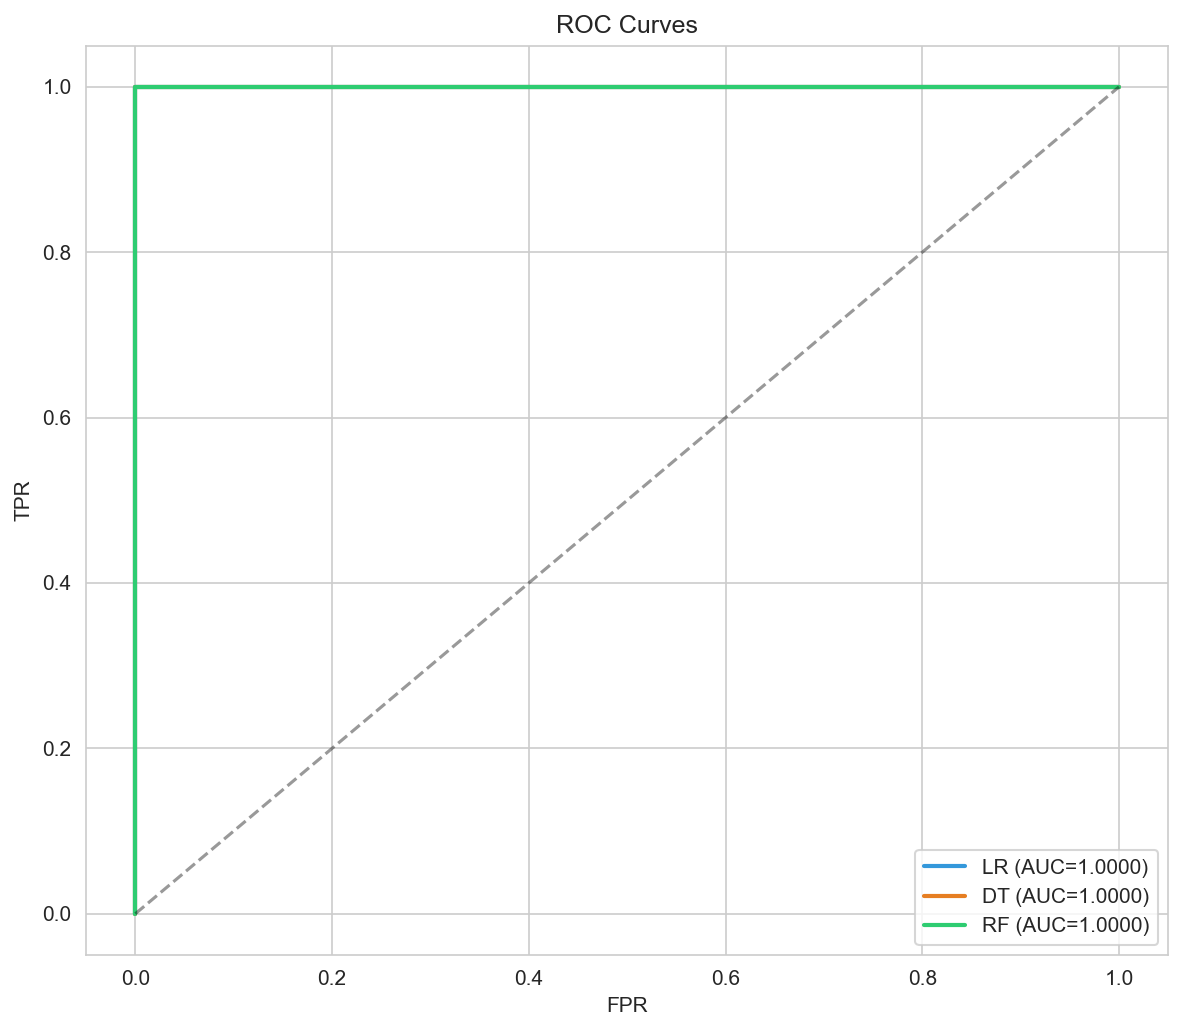
\includegraphics[width=0.62\linewidth]{fig_roc_curves.png}
  \caption{ROC curves on the PhiUSIIL test set. AUC = 1.0000 for LR, DT, and RF; GRU reaches 0.9999. All four lines overlap at this scale.}
  \label{fig:roc}
\end{figure}

\begin{figure}[ht]
  \centering
  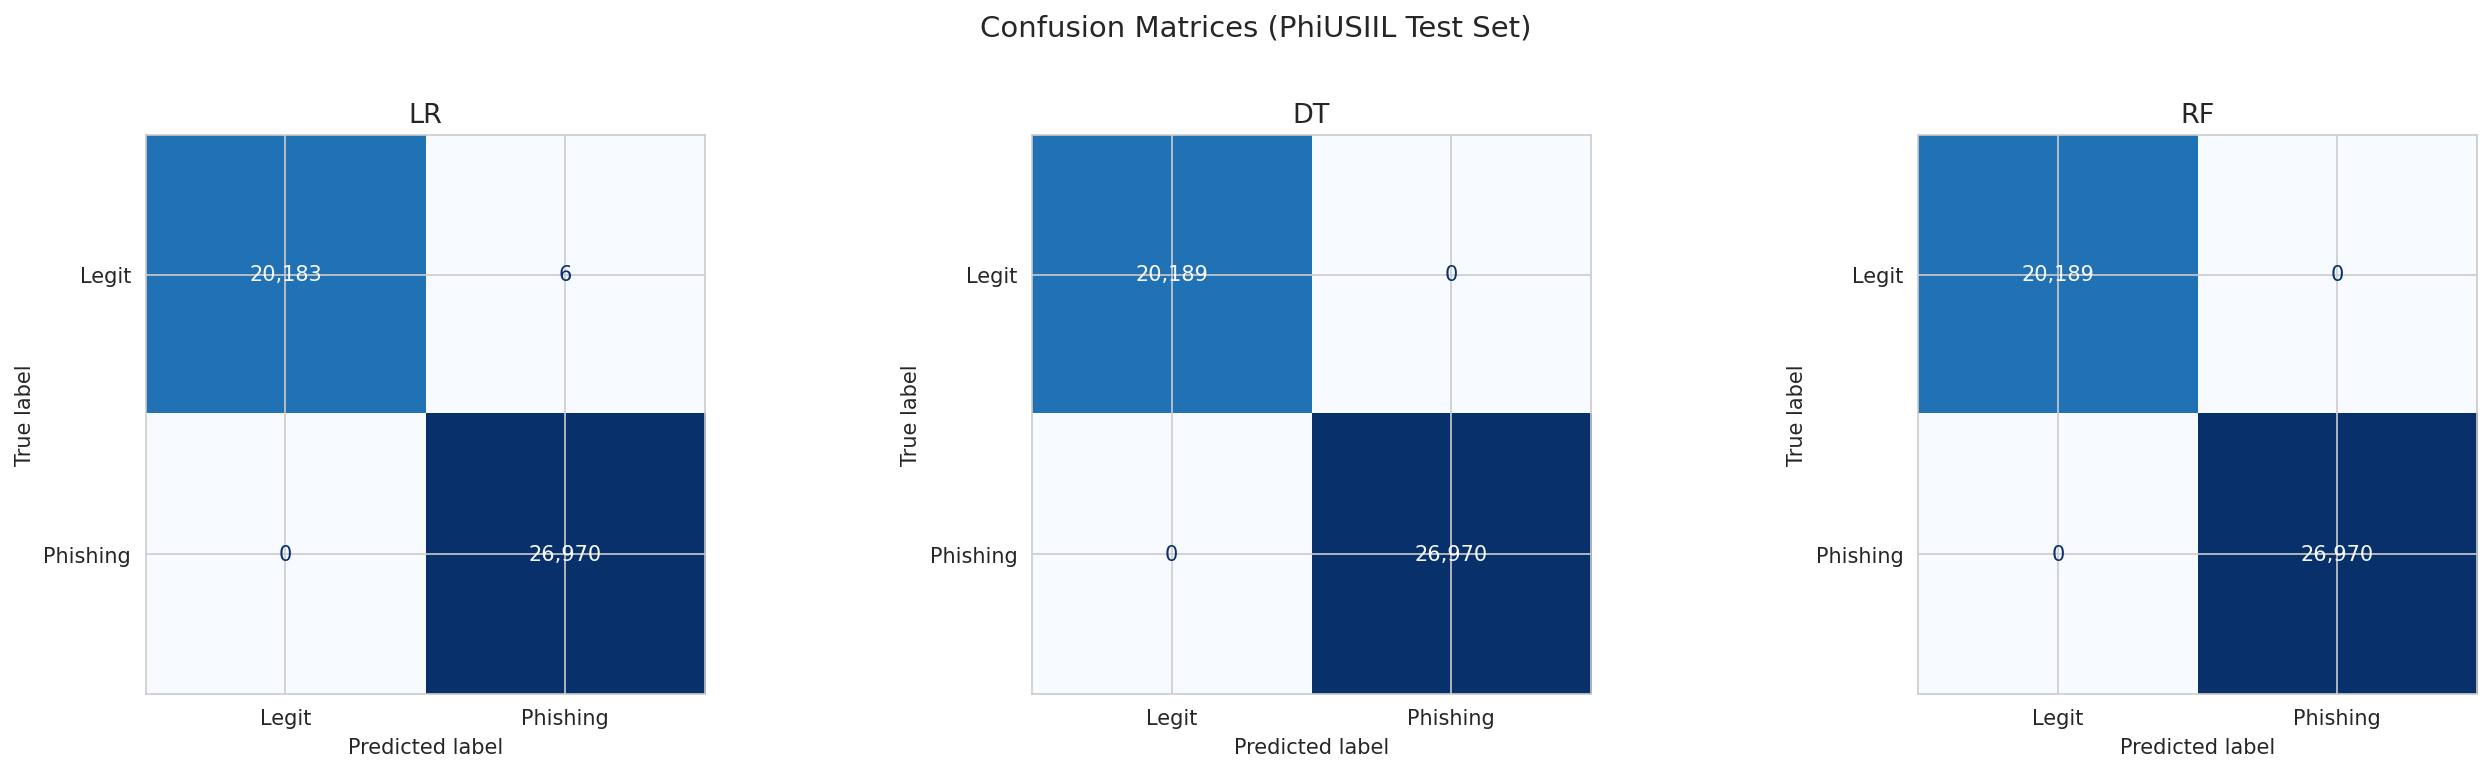
\includegraphics[width=0.86\linewidth]{fig_confusion_matrices.png}
  \caption{Confusion matrices on the PhiUSIIL test set (20,189 legitimate; 26,970 phishing). DT and RF are perfect; LR has 6 false positives.}
  \label{fig:cm}
\end{figure}

\subsection{UCI Phishing Websites Results}

Table~\ref{tab:uci} shows results on UCI, where the scores spread out and model ranking becomes clear.

\begin{table}[ht]
\caption{Test-set performance on UCI Phishing Websites ($n_\text{train} = 8{,}844$; $n_\text{test} = 2{,}211$).}
\label{tab:uci}
\centering
\begin{tabular}{lccccc}
\toprule
Model & Accuracy & Precision & Recall & F1 & AUC \\
\midrule
Logistic Regression     & 0.9281 & 0.9344 & 0.9010 & 0.9174 & 0.9785 \\
Decision Tree           & 0.9507 & 0.9476 & 0.9408 & 0.9442 & 0.9853 \\
GRU                     & 0.9548 & 0.9596 & 0.9490 & 0.9498 & 0.9901 \\
\textbf{Random Forest}  & \textbf{0.9769} & \textbf{0.9804} & \textbf{0.9673} & \textbf{0.9738} & \textbf{0.9964} \\
\bottomrule
\end{tabular}
\end{table}

RF leads on every metric.
The F1 gap to LR is 5.6 points; to DT it is 2.9 points.
GRU lands between DT and RF at F1 = 0.950, a reasonable result for a sequential architecture applied to non-sequential tabular data.
LR's recall of 0.90 is the most practically significant weak spot: missing 1 in 10 phishing pages is a real problem for a security tool.
Figure~\ref{fig:cross} shows both datasets side by side, making the ceiling effect on PhiUSIIL and the true spread on UCI visible at once.

\begin{figure}[ht]
  \centering
  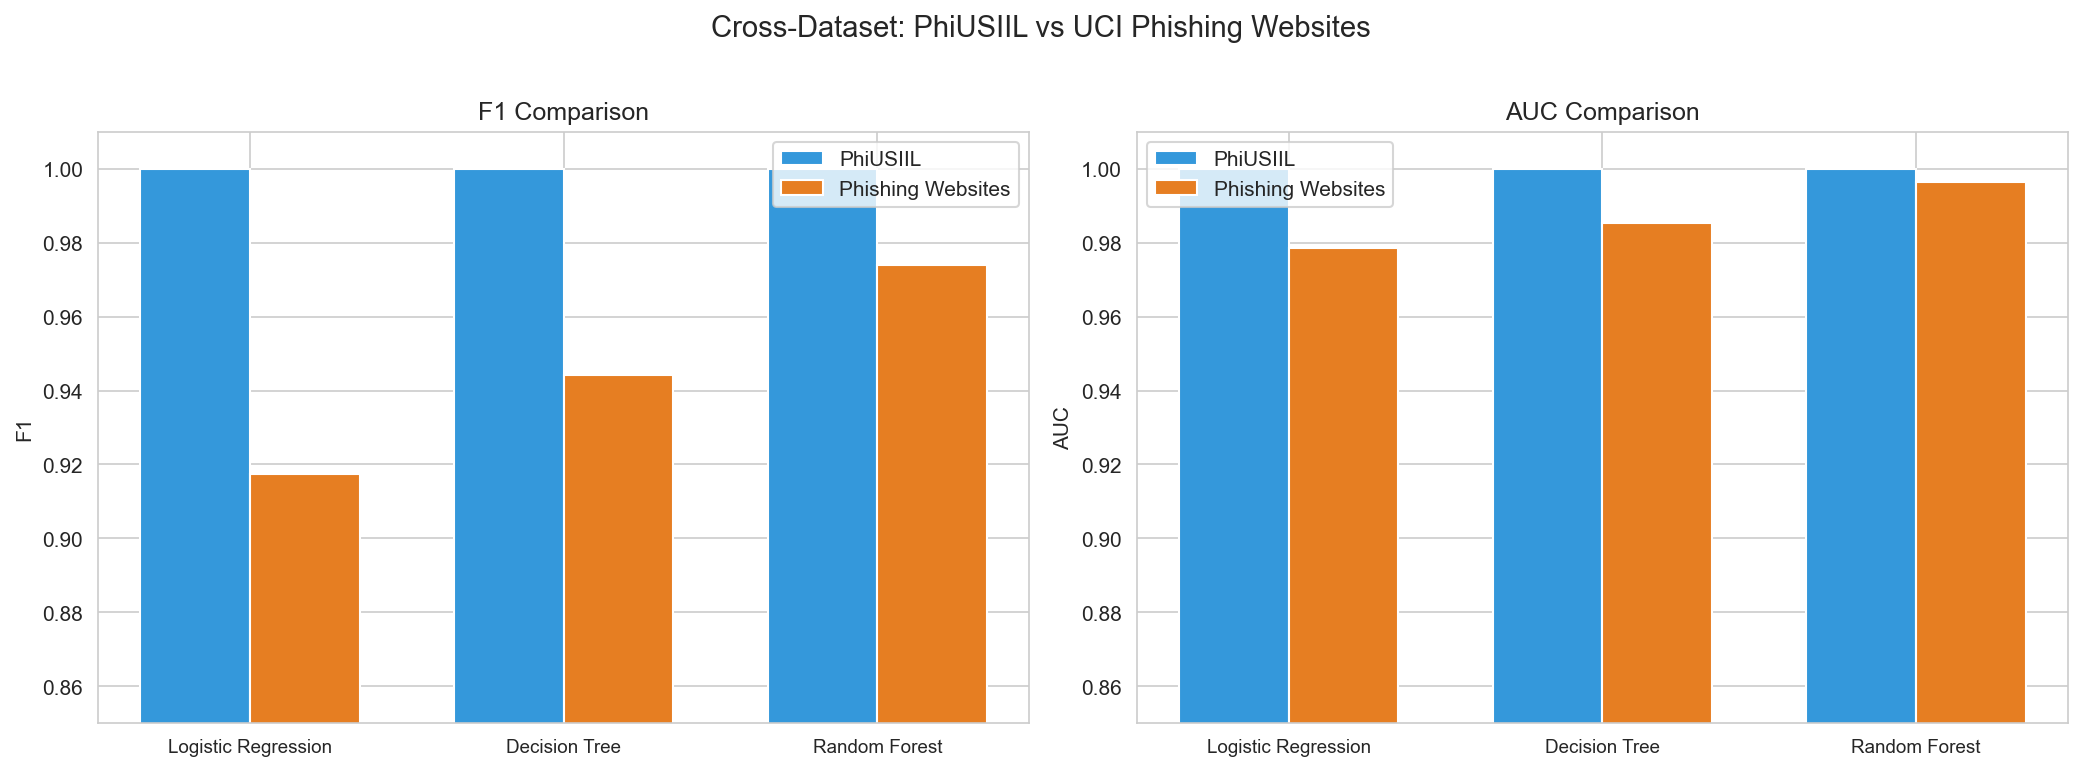
\includegraphics[width=0.82\linewidth]{fig_cross_dataset.png}
  \caption{F1 and AUC across both datasets. PhiUSIIL bars (blue) are near 1.0 for all models. UCI bars (orange) show the actual spread.}
  \label{fig:cross}
\end{figure}

\subsection{Feature Analysis}

Figure~\ref{fig:rf_imp} shows the top-15 most important features for the Random Forest.
\texttt{URLSimilarityIndex} (0.1974) and \texttt{NoOfExternalRef} (0.1656) stand out by a wide margin.
Behind them, a second group of page-size features follows: \texttt{LineOfCode} (0.1314), \texttt{NoOfImage} (0.1125), \texttt{NoOfSelfRef} (0.0869), and \texttt{NoOfJS} (0.0754).
These all make intuitive sense: legitimate sites tend to link out heavily and have fully-built pages, while a minimal phishing form has almost none of that structure.

\begin{figure}[ht]
  \centering
  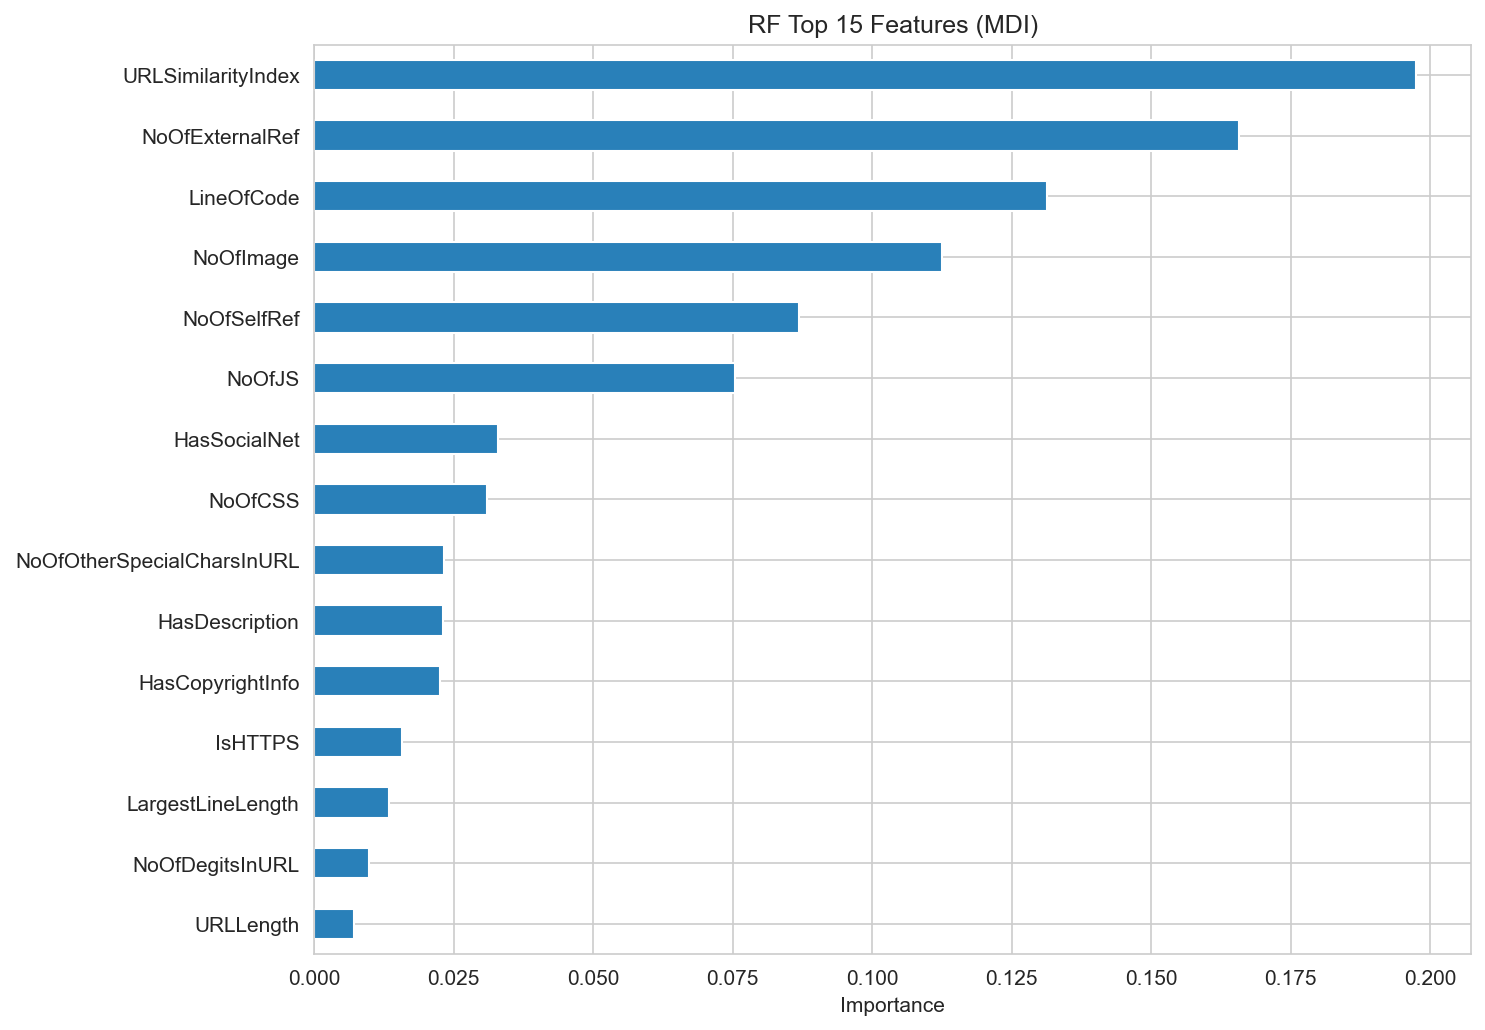
\includegraphics[width=0.72\linewidth]{fig_rf_feature_importance.png}
  \caption{RF top-15 feature importances. \texttt{URLSimilarityIndex} and \texttt{NoOfExternalRef} dominate; page-volume features form a clear second tier.}
  \label{fig:rf_imp}
\end{figure}

\subsection{Error Analysis}

Figure~\ref{fig:errors} shows the false positive and false negative counts for each model on UCI.
LR produces 62 false positives and 97 false negatives; DT has 51 and 58; RF drops to 19 and 32.
The right panel of Figure~\ref{fig:errors} shows the mean feature values of LR's false negatives against the phishing pages it caught correctly.
The gap on \texttt{SSLfinal\_State} is the largest of any feature: missed pages average 0.619 (mostly legitimate indicator) while caught pages average $-0.618$ (mostly phishing indicator).
\texttt{URL\_of\_Anchor} and \texttt{Request\_URL} also differ sharply (0.175 vs $-0.708$, and 0.485 vs $-0.162$ respectively).
The pages LR misses look legitimate on the very signals that modern phishing kits are designed to mimic.

\begin{figure}[ht]
  \centering
  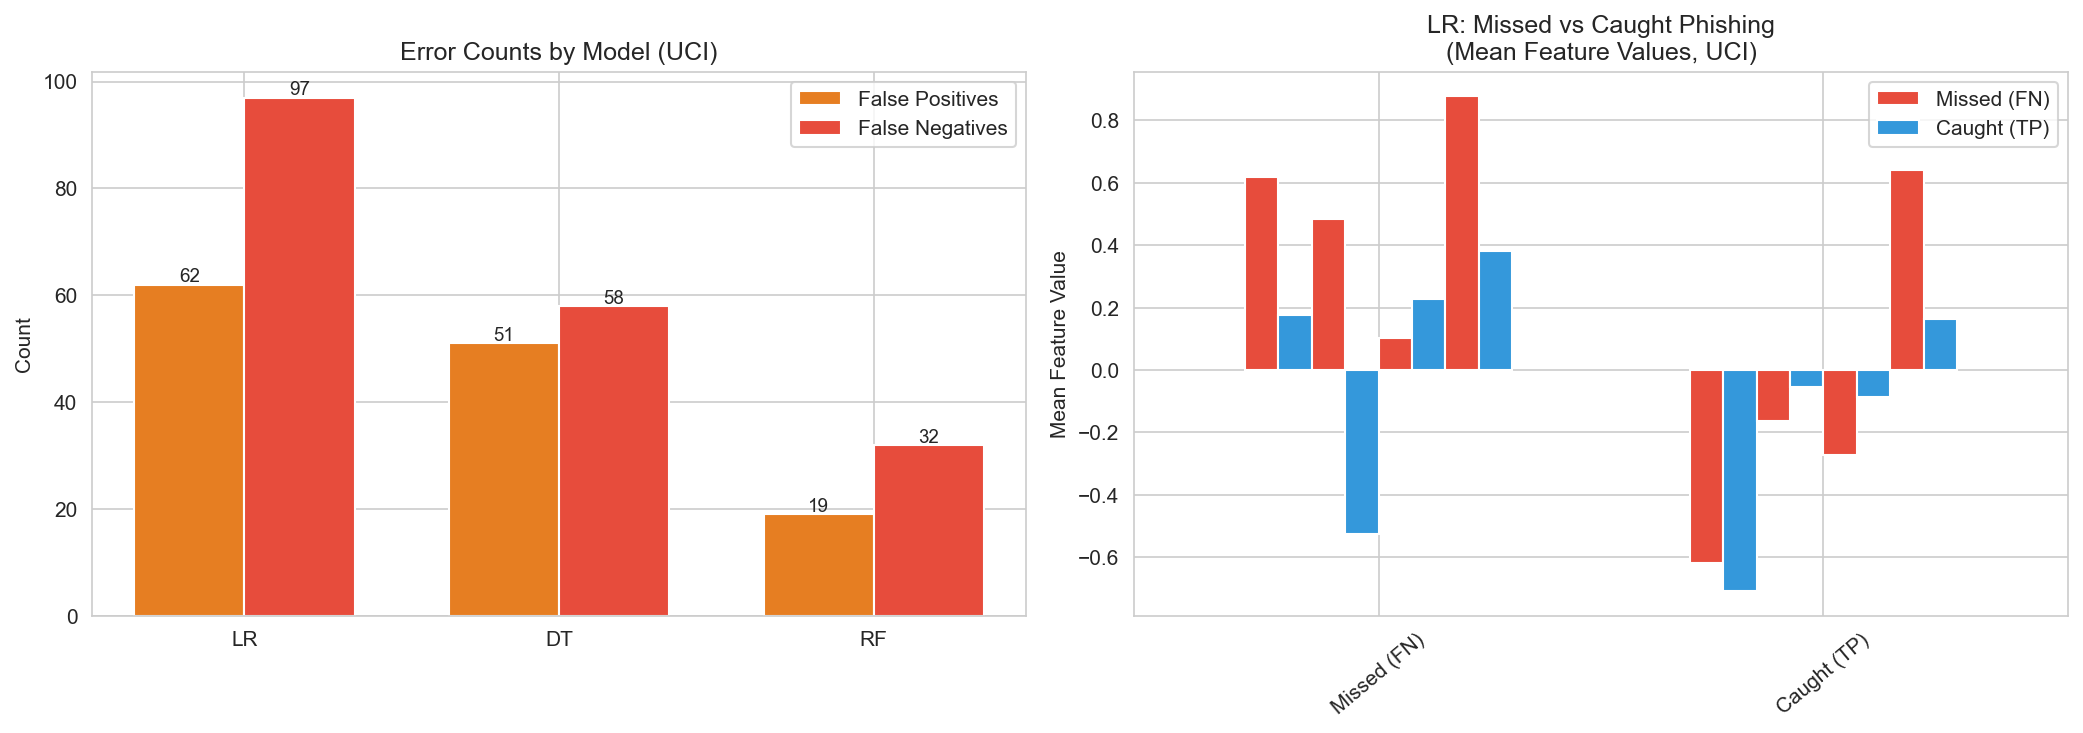
\includegraphics[width=\linewidth]{fig_error_analysis.png}
  \caption{Left: false positive and false negative counts per model on UCI. Right: mean feature values for LR's missed phishing pages (red) versus correctly caught phishing pages (blue). The gap on \texttt{SSLfinal\_State} is the largest, confirming that LR struggles most with phishing pages that have valid SSL.}
  \label{fig:errors}
\end{figure}

To make this concrete, Table~\ref{tab:fn_examples} shows two representative false negatives from the UCI test set, both phishing pages that LR called legitimate while RF caught correctly.
All values follow the dataset encoding: 1 = legitimate indicator, 0 = suspicious, -1 = phishing indicator.

\begin{table}[ht]
\caption{Two representative false negatives from the UCI test set. LR classified both as legitimate; RF classified both correctly as phishing. Encoding: 1 = legitimate, 0 = suspicious, -1 = phishing.}
\label{tab:fn_examples}
\centering
\small
\begin{tabular}{lcc}
\toprule
Feature & Sample A & Sample B \\
\midrule
\texttt{SSLfinal\_State}            & \phantom{-}1 & \phantom{-}1 \\
\texttt{URL\_of\_Anchor}            & \phantom{-}1 & \phantom{-}0 \\
\texttt{Request\_URL}               & \phantom{-}1 & \phantom{-}1 \\
\texttt{Domain\_registeration\_length} & $-1$       & $-1$ \\
\texttt{having\_Sub\_Domain}        & \phantom{-}1 & \phantom{-}0 \\
\texttt{web\_traffic}               & \phantom{-}1 & \phantom{-}0 \\
\texttt{SFH}                        & $-1$          & $-1$ \\
\texttt{having\_IP\_Address}        & \phantom{-}1 & \phantom{-}0 \\
\midrule
LR prediction  & Legitimate & Legitimate \\
RF prediction  & Phishing   & Phishing   \\
True label     & Phishing   & Phishing   \\
\bottomrule
\end{tabular}
\end{table}

\textbf{Sample A} looks legitimate on all three of the most discriminating features.
The page has a valid SSL certificate (\texttt{SSLfinal\_State} = 1), anchor links that appear legitimate (\texttt{URL\_of\_Anchor} = 1), and resources loaded from the same domain (\texttt{Request\_URL} = 1).
Those three features carry enough positive weight in LR's sum to override the freshly registered domain and external form submission.
RF catches it because the combination of a new domain, external form handling, and legitimate-looking surface signals is a pattern its trees have learned to flag as suspicious even when the individual signals point in different directions.

\textbf{Sample B} is a newer page with valid SSL but suspicious anchor URLs (\texttt{URL\_of\_Anchor} = 0) and no web traffic.
For LR, \texttt{SSLfinal\_State} = 1 is still the strongest signal in the weighted sum and it tips the balance toward legitimate.
RF and the GRU both catch it correctly; the GRU in particular catches both sample cases, which suggests the recurrent structure is picking up on the same inter-feature dependency that RF exploits: valid SSL coexisting with missing traffic and a suspicious domain registration is a combination that a linear model cannot easily represent.

These two examples illustrate why the recall gap between LR and RF is not just a number.
It reflects a real structural difference: LR is vulnerable to phishing pages that invest in looking legitimate at the domain and SSL level, while RF and the GRU are better at recognizing when those surface-level signals co-occur with the kind of HTML behavior that a real site would not have.

\section{Discussion}
\label{sec:discussion}

The near-perfect PhiUSIIL results say something about the data, not just the models.
The feature set likely has at least one dominant separating signal---\texttt{URLSimilarityIndex}---that is strong enough for even LR to find it.
This means PhiUSIIL is essentially a solved benchmark for classical ML and is a poor place to rank models against each other.
UCI is where the real comparison happens.

On UCI, the $\{-1, 0, 1\}$ feature encoding suits tree-based splits naturally, which helps DT and RF.
LR has to approximate threshold behavior with a weighted sum, which is less efficient here.
GRU's mid-table finish is informative: it does better than DT despite being applied to non-sequential data, suggesting it is learning useful non-linear combinations, but the tree ensemble still extracts more from the same features.
The error analysis sharpens the picture further---all four models share a common failure mode on pages engineered to look structurally legitimate, which no amount of model tuning on existing features will fully resolve.

\section{Limitations}
\label{sec:limitations}

Both datasets are single-time snapshots split randomly.
A proper generalization test would use older data for training and newer phishing campaigns for testing; neither dataset is set up for that.
Many high-importance features also require fetching and rendering the actual page, which introduces latency that would need to be managed in a real deployment.

The GRU used here is a basic adaptation of a sequential model to non-sequential tabular data.
A multi-layer perceptron or attention-based model would be a more principled deep learning baseline.
Finally, two datasets are better than one but not enough to make a strong generalization claim; data from multiple time periods and attack campaign types would give a more complete picture.

\section{Conclusion}
\label{sec:conclusion}

I compared Logistic Regression, Decision Tree, Random Forest, and a GRU on two phishing detection datasets.
On PhiUSIIL all four hit near-perfect performance because the feature set makes classification nearly trivial.
On UCI the real ranking appears: RF at F1 = 0.974, GRU at 0.950, DT at 0.944, and LR at 0.917.

The word cloud of LR feature weights and the error analysis of UCI misclassifications both tell the same story: \texttt{URLSimilarityIndex} is the dominant signal on PhiUSIIL, and on UCI the hardest cases are pages that look structurally legitimate because attackers have learned to mimic the cues these models trust.
A benchmark giving perfect scores to a linear model is too easy to reveal anything interesting about model differences.
The harder dataset, and the specific cases that every model gets wrong, are where the useful findings actually are.

\newpage
\begin{thebibliography}{10}
\small

\bibitem{prasad2024}
Prasad, A., \& Chandra, R. (2024).
PhiUSIIL: Phishing URL/Website Identification using Intrinsic and Implicit Latent features.
\textit{Computers \& Security}.

\bibitem{uci_phiusiil}
UCI ML Repository. PhiUSIIL Phishing URL Dataset (2024).
\url{https://archive.ics.uci.edu/dataset/967/phiusiil+phishing+url+dataset}

\bibitem{uci2015}
UCI ML Repository. Phishing Websites Dataset (2015).
\url{https://archive.ics.uci.edu/dataset/327/phishing+websites}

\bibitem{tang2021}
Tang, L., \& Mahmoud, Q.~H. (2021).
A survey of machine learning-based solutions for phishing website detection.
\textit{Machine Learning and Knowledge Extraction}, 3(3), 672--694.

\bibitem{zieni2023}
Zieni, R., Massari, L., \& Calzarossa, M.~C. (2023).
Phishing or not phishing? A survey on the detection of phishing websites.
\textit{IEEE Access}, 11.

\bibitem{whittaker2010}
Whittaker, C., Ryner, B., \& Nazif, M. (2010).
Large-scale automatic classification of phishing pages.
In \textit{NDSS}.

\bibitem{cho2014}
Cho, K., van Merrienboer, B., Gulcehre, C., Bahdanau, D., Bougares, F., Schwenk, H., \& Bengio, Y. (2014).
Learning phrase representations using RNN encoder-decoder for statistical machine translation.
In \textit{EMNLP}.

\bibitem{apwg2023}
Anti-Phishing Working Group (2023).
Phishing Activity Trends Report, Q4 2023.
\url{https://apwg.org/trendsreports/}

\bibitem{sklearn}
Pedregosa, F., et al.\ (2011).
Scikit-learn: Machine Learning in Python.
\textit{JMLR}, 12, 2825--2830.

\end{thebibliography}

\end{document}
